\documentclass{beamer}

\mode<presentation>
{
  \usetheme{CambridgeUS}
  \usecolortheme{beaver}
  \usefonttheme{default}
  \setbeamertemplate{navigation symbols}{}
  \setbeamertemplate{caption}[numbered]
}

\usepackage[english]{babel}
\usepackage[utf8x]{inputenc}
\usepackage{color}
\usepackage{minted}
% \usemintedstyle{native}

\title[IAP-2017]{Using Computational Resources in Optimization and Statistics}
\author{Sébastien Martin}
\institute{MIT}
\date{Tuesday 01/24/2017}

\begin{document}

\begin{frame}
  \titlepage
\end{frame}


\section{Introduction}

\begin{frame}{Heavy Computations}
  In Optimization and Statistics, we often need a lot of computational power:
  \begin{itemize}
    \item Machine Learning on large datasets
    \item Hard optimization problems, mixed integer programming
  \end{itemize}
  \pause
  Or repetitive computations:
  \begin{itemize}
    \item Parameter tuning
    \item Benchmarking
  \end{itemize}
\end{frame}

\begin{frame}{Limitations of a Personal Computer}
  Using your personal computer may seem simple, but there are serious limitations:
  \begin{itemize}
    \item<1-> Limited \alert{memory} (Big Data, large matrices...)
    \item<2-> Limited \alert{computational power}.
    \item<3-> Limited \alert{number of machines}/cores.
    \item<4-> Limited \alert{time} available. (you want to use your laptop for other things too..)
  \end{itemize}
\end{frame}

\begin{frame}{How does it work : using a remote computer}
  \begin{figure}
    
\includegraphics[width=\linewidth]{figures/iap2017-diagram1}
  \end{figure}
  An interactive remote control is the easiest way to use another computer.
  \begin{itemize}
    \item We use \alert{SSH} (see lecture 1) to control a terminal on a remote machine through our computer.
    \item We can use the \alert{console} to do almost anything on the remote computer: create files, run a program, use Julia...
    \item It is also possible to use graphical softwares like \alert{R-Studio or Matlab}.
    \item It works with any computer, including your own machines.
  \end{itemize}
\end{frame}

\begin{frame}{How does it work : using a cluster}
  \begin{figure}
    \only<1>{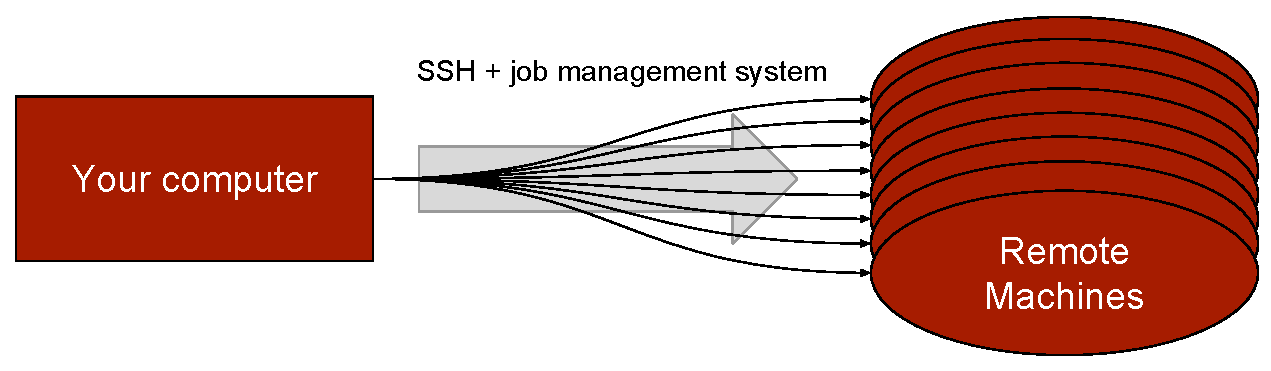
\includegraphics[width=\linewidth]{figures/iap2017-diagram2}}
    \only<2>{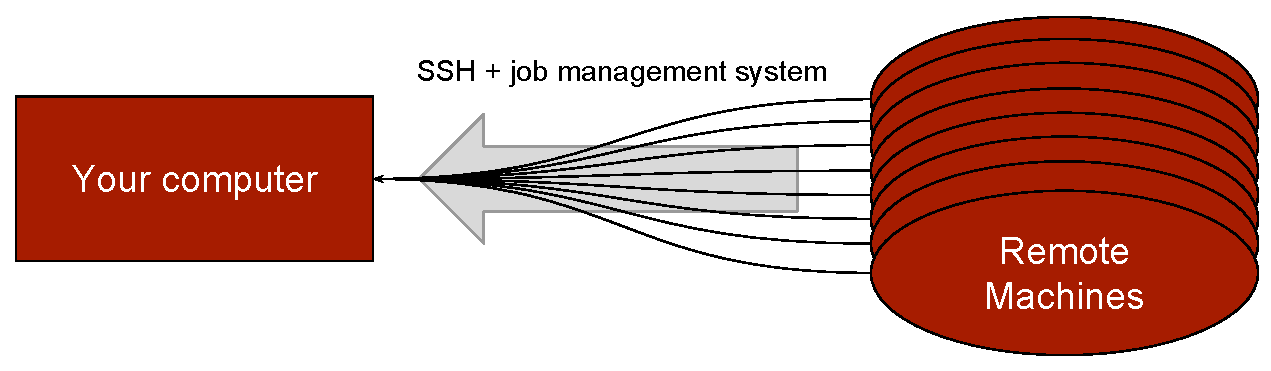
\includegraphics[width=\linewidth]{figures/iap2017-diagram3}}
  \end{figure}
  When a computing cluster is available, we can run multiple ``jobs'' thanks to a \alert{job management system}.
  \begin{itemize}
    \item Allows us to use multiple remote machines, manages demand and resources available.
    \item Different job management systems exist, I will use the example of Slurm, available to Sloan and ORC students on the cluster \alert{Engaging}.
    \item More complex to use, but far more \alert{powerful}.
  \end{itemize}
\end{frame}

\begin{frame}{Resources}
  There are several ways to have access to a remote computer or a cluster.
  \begin{itemize}
    \item Another personal computer you own.
    \item Athena at MIT.
    \item Resources of your department/lab (Engaging at Sloan).
    \item Paying options: cloud computing (Amazon AWS, Google Cloud Computing...).
  \end{itemize}
\end{frame}

\begin{frame}{Why Should I Use this}
  For research:
  \begin{itemize}
    \item Tackle \alert{bigger problems} in Stats and Optimization.
    \item \alert{Parallelize} your computations (parameter grid search in ML for example)!
    \item Longer computational times: \alert{run overnight} or for a whole week!
    \item \alert{Bigger Datasets} become manageable.
    \item Can be very simple to use with interactive sessions (\alert{RStudio}...)
  \end{itemize}
  In general:
  \begin{itemize}
    \item \alert{Useful skill}, at the age of cloud computing.
    \item \alert{Good practice} to learn how to use console (and GitHub).
  \end{itemize}
\end{frame}

\section{Using a Remote Machine}
\begin{frame}{What Machine? Engaging}
  Engaging is a powerful computing cluster for MIT Sloan affiliates, request an account at \texttt{stshelp@mit.edu}. It uses the job management system \alert{Slurm}, that we will use in this presentation.
  \vspace{1cm}
  \begin{block}{Connecting to Engaging}
    \begin{description}
      \item[Hostname] \texttt{eosloan1.mit.edu}
      \item[Username] MIT Kerberos username (not your email address)
      \item[Password] MIT Kerberos password
    \end{description}
    \texttt{wikis.mit.edu/confluence/display/sloanrc/Engaging+Platform}
  \end{block}
\end{frame}

\begin{frame}{What Machine? Athena}
  Any MIT affiliate can access the Athena distributed computing environment, you can use it to follow if you do not have access to Engaging.
  \vspace{1cm}
  \begin{block}{Connecting to Athena}
    \begin{description}
      \item[Hostname] \texttt{athena.dialup.mit.edu}
      \item[Username] MIT Kerberos username (not your email address)
      \item[Password] MIT Kerberos password
    \end{description}
    \texttt{http://web.mit.edu/dialup/www/ssh.html}
  \end{block}
\end{frame}

\begin{frame}[fragile]{SSH}
  As seen in Lecture 1, you can connect to the remote machine through SSH:
  \begin{minted}{console}
[sebastien@seblaptop ~]$ ssh semartin@eosloan1.mit.edu
Password:
[semartin@eosloan1 ~]$
  \end{minted}
  \invisible<1>{
  \begin{block}{Tip}
    If you connect regularly to the same remote, you can set up a \alert{password-less login} (see Google). You can also set-up an alias instead of typing the full address each time.
  \end{block}}
\end{frame}

\begin{frame}[fragile]{SSH}
  As seen in Lecture 1, you can connect to the remote machine through SSH:
  \begin{minted}{console}
[sebastien@seblaptop ~]$ ssh semartin@athena.dialup.mit.edu
Password:
semartin@buzzword-bingo:~$
  \end{minted}
 \begin{block}{Tip}<2>
    If you connect regularly to the same remote, you can set up a \alert{password-less login} (see Google). You can also set-up an alias instead of typing the full address each time.
  \end{block}
\end{frame}

\begin{frame}[fragile]{Using the Terminal}
    Once you are connected to the remote machine, you can use the terminal to interact with it:
    \begin{minted}{console}
[semartin@eosloan1 ~]$ pwd
/home/semartin
[semartin@eosloan1 ~]$ mkdir testfolder
[semartin@eosloan1 ~]$ cd testfolder
[semartin@eosloan1 testfolder]$ pwd
/home/semartin/testfolder
    \end{minted}
\end{frame}

\begin{frame}[fragile]{Using Git/GitHub to Synchronize Code}
    If you need to run code on the remote machine, an elegant way is to use git and GitHub:
    \begin{figure}
      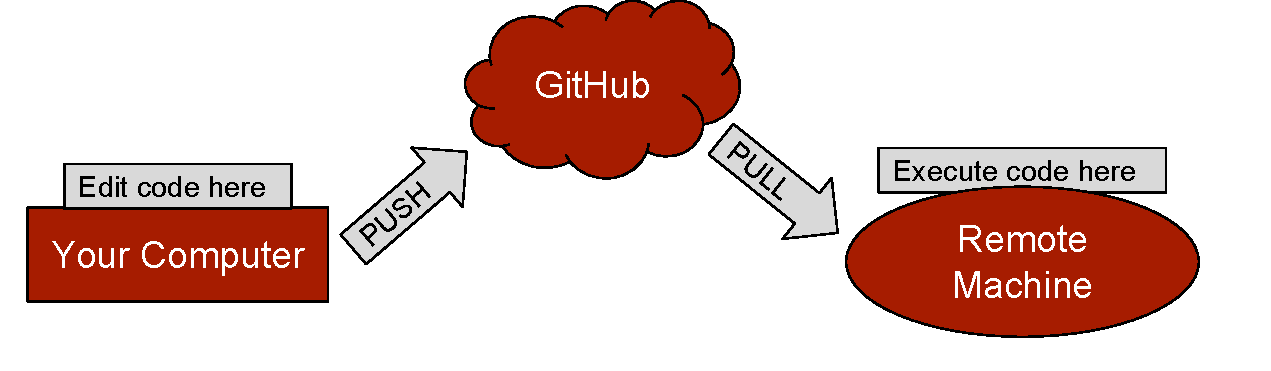
\includegraphics[width=\linewidth]{figures/iap2017-diagram4}
    \end{figure}
    \pause
    \begin{minted}{console}
[semartin@eosloan1 testfolder]$ git clone \
> https://github.com/sebmart/IAP2017-computing-ressources.git
Cloning into 'IAP2017-computing-ressources'...
    \end{minted}
\end{frame}

\begin{frame}[fragile]{Using Screen to Keep your Session}
  By default, your session is lost when your ssh connection ends. \alert{Linux Screen} can be used to close the connection while letting things run on the remote, and restart where you were.

  \pause

  \vspace{0.5cm}

  \alert{Start screen session}: similar to starting a new terminal

  \begin{minted}{console}
[semartin@eosloan1 testfolder]$ screen
  \end{minted}

  \alert{Detach the screen session} before closing SSH: \texttt{Ctrl+A then D}: goes back to previous terminal. Then close the SSH connection (\texttt{Ctrl+D})

  \vspace{0.3cm}

  Restart the SSH connection and \alert{re-attach your screen session} as it was before:
  \begin{minted}{console}
[semartin@eosloan1 testfolder]$ screen -r
  \end{minted}
\end{frame}

\begin{frame}[fragile]{Useful commands}
  \begin{itemize}
  \item Downloading from the Internet (useful to install software, or download datasets ): \alert{wget}
  \begin{minted}{console}
$ wget http://data.com/awesomedata.csv
  \end{minted}
  \item Transferring files between the local and remote machines: Secure Copy \alert{scp}
  \begin{minted}{console}
$ scp mylocalfile.txt semartin@eosloan1.mit.edu:~
  \end{minted}

  \end{itemize}

  \pause

  \begin{block}{For advanced users}
    Use a search engine to learn more about this !
    \begin{itemize}
      \item \alert{screen} has lots of other advanced features (multiple windows...).
      \item \alert{tmux} (terminal multiplexer) is like screen with lots of additional functionalities (panes...)
      \item \alert{sshfs} allows you to access the files of the remote machine as if they were on your own (quite magic)!
    \end{itemize}

  \end{block}
\end{frame}

\section{Running Jobs on a Cluster}

\end{document}
